\chapter{Oscillations}
\begin{center}
    \includegraphics[width=0.25\textwidth,page=20]{../images/SHM/SHMCropped.pdf}
    \captionsetup{type=figure}
    \caption[figure]{\ref{Simple harmonic motion} Simple harmonic motion.}
\end{center}
\begin{itemize}
    \item \emph{Simple harmonic motion} is defined as the motion of a body whose acceleration is directly proportional to its displacement from a fixed point (equilibrium position) and is always directed towards that fixed point.
    \begin{example}{}{}
        Describe the restoring force that gives rise to oscillations in a simple pendulum.
        \begin{figure}[H]
            \centering
            \includegraphics[width=0.2\textwidth]{../images/simple-pendulum-restoring-force.jpg}
            \caption{A simple pendulum.}
            \label{fig:simple-pendulum-restoring-force}
        \end{figure}
        \rule{20cm-137.0549pt-25pt}{0.05mm}

        \vspace{0.5\baselineskip} The restoring force is the \textcolor{green!70!black}{tangential component of the weight} of the bob, which is normal to the string and points towards the equilibrium position --- where the pendulum is hanging vertically. 

        \vspace{0.5\baselineskip} \emph{Note.} the \textcolor{red}{tension} in the string does not provide the restoring force, since there is no component of tension along the tangential direction of motion.
    \end{example}
    \item A \emph{freely oscillating} system oscillates at its own \emph{natural frequency} without \emph{external} influences other than the \emph{initial impulse when displaced} from its equilibrium position, with \emph{no dissipation} of energy.
    \item \emph{Damped oscillations} are oscillations in which the amplitude diminishes with time as a result of \emph{dissipative forces} that reduce the total energy of the oscillations.
    \item \emph{A forced oscillating system} is one that is driven by an \emph{external periodic driver}. There is \emph{continuous energy input} to the oscillating system by the driver, and the system \emph{oscillates at the driver's frequency}. 
    \item \emph{Resonance} is a phenomenon in which there is \emph{maximum transfer of energy} from the driver to the oscillating system in a \emph{forced oscillation}. The oscillating system achieves \emph{maximum amplitude} during resonance. For an \emph{undamped system}, resonance occurs when the \emph{driving frequency} is \emph{equal} to its \emph{natural frequency} of vibration.
\end{itemize}
\begin{itemize}[label=\(\square\)]
    \item \begin{tabular}{|Sc|Sc|Sc|Sc|Sc|}
        \hline
        \multirow{2}{*}[-1em]{\(\begin{aligned}
            v=\pm \omega \sqrt{x_0^2-x^2}
        \end{aligned}\)}&\multirow{2}{*}[-1em]{\(\begin{aligned}
            a=-\omega^2x
        \end{aligned}\)}& Spring-Mass & Pendulum\\
            &
            &
            \(\begin{aligned}
                \omega=\sqrt{\frac{k}{m}} 
                % \quad\&\quad T=2\pi\sqrt{\frac{m}{k}}
            \end{aligned}\)&
            \(\begin{aligned}
                \omega=\sqrt{\frac{g}{l}} 
                % \quad\&\quad T=2\pi\sqrt{\frac{l}{g}}
            \end{aligned}\)
        \\
        \hline
    \end{tabular}
    \begin{figure}[H]
        \centering
        \begin{subfigure}[c]{0.45\textwidth}
            \centering
            \includegraphics[page=2,width=\textwidth]{../images/SHM/SHM-too.pdf}
            \caption{Velocity against displacement.}
            \label{fig:SHM-graphs-v-x}
        \end{subfigure}%
        \begin{subfigure}[c]{0.45\textwidth}
            \centering
            \includegraphics[page=3,width=\textwidth]{../images/SHM/SHM-too.pdf}
            \caption{Acceleration against time.}
            \label{fig:SHM-graphs-a-x}
        \end{subfigure}%
        \caption{\ref{Simple harmonic motion graphs} Graphs for velocity and acceleration.}
        \label{fig:SHM-graphs-v-and-a-against-t}
    \end{figure}
    \item \begin{tabular}{|Sc|Sc|Sc|Sc|}
        \hline
    Variable
        &
    \(\begin{aligned}
        E_k
    \end{aligned}\)&
    \(\begin{aligned}
        E_p
    \end{aligned}\)&
    \(\begin{aligned}
            E_T
    \end{aligned}\)\\
    \hline
        Time 
        \(\begin{aligned}
            t
        \end{aligned}\)&
        \(\begin{aligned}
            \frac{1}{2}m\omega^2x_0^2\cos^2(\omega t)
        \end{aligned}\)&
        \(\begin{aligned}
            \frac{1}{2}m\omega^2x_0^2\sin^2(\omega t)
        \end{aligned}\)&
        \multirow{2}{*}[-1.8mm]{
            \(\begin{aligned}
            \frac{1}{2}m\omega^2x_0^2
            \end{aligned}\)
        }\\
        \cline{1-3}
        Displacement
        \(\begin{aligned}
            x
        \end{aligned}\)&
        \(\begin{aligned}
            \frac{1}{2}m\omega^2(x_0^2-x^2)
        \end{aligned}\)&
        \(\begin{aligned}
            \frac{1}{2}m\omega^2x^2
        \end{aligned}\)&
        \\
        \hline
    \end{tabular}
    \begin{figure}[H]
        \centering
        \begin{subfigure}[c]{0.45\textwidth}
            \centering
            \includegraphics[page=4,width=\textwidth]{../images/SHM/SHM-too.pdf}
            \caption{Kinetic/potential energies against time.}
            \label{fig:SHM-graphs-E-t}
        \end{subfigure}%
        \begin{subfigure}[c]{0.45\textwidth}
            \centering
            \includegraphics[page=1,width=\textwidth]{../images/SHM/SHM-too.pdf}
            \caption{Kinetic/potential energies against displacement.}
            \label{fig:SHM-graphs-E-x}
        \end{subfigure}%
        \caption{\ref{Simple harmonic motion graphs} Graphs for kinetic/potential energies.}
        \label{fig:SHM-graphs-E-t-and-E-x}
    \end{figure}
    \item Simple pendulums and mass spring systems can be approximated to be SHM when the angle of oscillation (\(\leq 20^\circ\)) and oscillation amplitude are small, respectively.
    \item \begin{tabular}{|Sc|Sc|Sc|Sc|}
        \hline
        & In Phase & Antiphase & Out of Phase\\
        \hline
        \(\Delta \phi\)/rad & 0 & \(\pi\) & nonzero
        \\
        \hline
    \end{tabular}
    \item When damping increases:
    \begin{itemize}[label=\(\circ\)]
        \item Amplitude at \emph{all} frequencies decreases.
        \item (Resonance) frequency at max amplitude shifts gradually to lower frequencies.
        \item Peak (max amplitude) becomes flatter.
    \end{itemize}
    \begin{figure}[H]
        \centering
        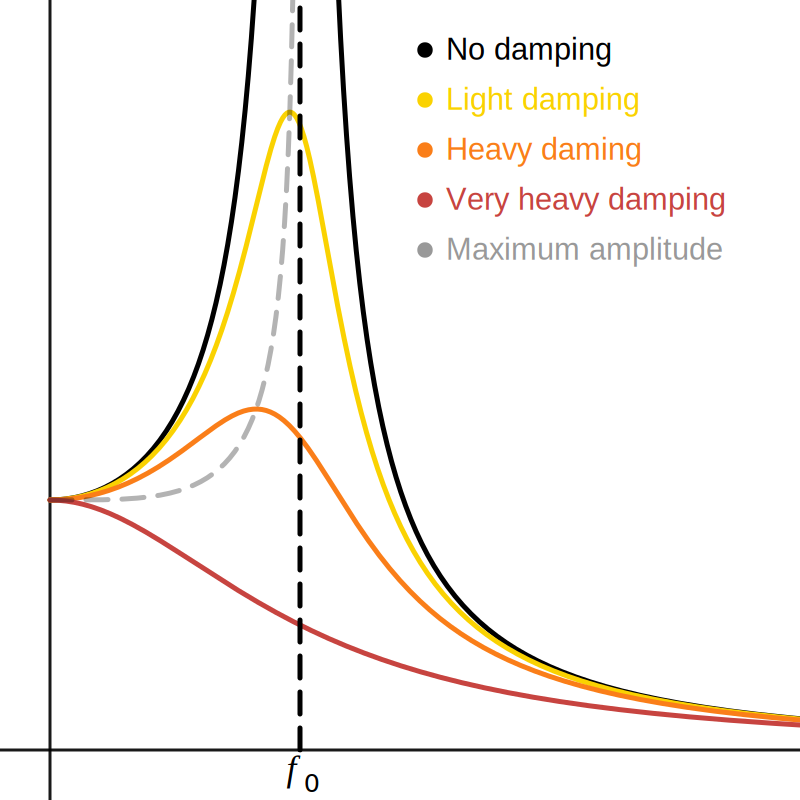
\includegraphics[width=0.5\textwidth]{../images/SHM/Amplitude-vs-frequency-graph.pdf}
        \caption{\ref{Simple harmonic motion amplitude-vs-frequency graph} The graph of amplitude against frequency, as damping increases. The resonance frequency is denoted by \(f_0\).}
        \label{fig:SHM-graphs-A-f}
    \end{figure}
    \item When drawing the displacement-time graph of a underdamped oscillator, we must show the exponential decay in amplitude:
    \begin{figure}[H]
        \centering
        \includegraphics{../images/light-damping/light-damping.pdf}
        \caption{\ref{source:underdamped} The displacement-time graph of an underdamped oscillator}
        \label{fig:underdamped}
    \end{figure}
\end{itemize}
\begin{example}{}{}
    The variation with time \(t\) of the total vertical displacement \(y\) of the mass \(M\) is shown in Figure \ref{fig:no-damping-to-light-damping}, when the oscillations are undamped. On Figure \ref{fig:no-damping-to-light-damping}, sketch the variation of time \(t\) of the total vertical displacement \(y\) of mass \(M\) for \textbf{three} complete, lightly damped oscillations of the mass.
    \begin{itemize}[label={--}]
        \item Same constant period \hspace*{\fill} [1]
        \item Gradual/continuous decrease in amplitude \hspace*{\fill} [1]
        \item Three complete cycles
    \end{itemize}
    \begin{figure}[H]
        \centering
        \includegraphics{../images/light-damping/untolight.pdf}
        \caption{\ref{Me} Changes to the displacement-time graph going from no damping to \textcolor{blue}{light damping}.}
        \label{fig:no-damping-to-light-damping}
    \end{figure}
\end{example}
(Ideal) Isolated spring systems are in simple harmonic motion, but spring systems in general need not be in simple harmonic motion.
\begin{example}{spring systems are not \emph{always} in simple harmonic motion.}{}
    Consider when a mass \(m\) is dropped onto a massless spring, that is at its equilibrium position. Assume that the mass does not rebound; the spring-mass system moves as one body after the initial collision occurs.
    \begin{figure}[H]
        \centering
        \includegraphics[width=0.25\textwidth]{../images/mass-spring system.jpg}
        \caption{An illustration of the spring-mass system aforementioned.}
        \label{fig:spring-mass-system}
    \end{figure}
    Then, the net force on the spring-mass system is \(W-F_{\text{spring}}=mg-kx\). Hence, the acceleration of the spring-mass system is \(g-(kx/m)\not\propto x\). i.e. the system does not move in simple harmonic motion.
\end{example}
(Regardless, the maximum speed occurs at the point where \(\text{net }F=0\).)